\documentclass{slides-style}

\slidetitle{Visual languages and their usage in IDEs}{29.12.2022}

\begin{document}

    \begin{frame}[plain]
        \titlepage
    \end{frame}

    \begin{frame}
        \frametitle{Visual Languages: big hopes}
        \begin{itemize}
            \item First visual languages --- 1970s, mainly for architecture
            \begin{itemize}
                \item Much like blueprints in ``classical'' engineering
            \end{itemize}
            \item ``CASE boom'' in 1990s --- visual languages as next generation of high-level languages
            \item UML, RUP --- 1995
            \item But then came Agile methodologies
        \end{itemize}
    \end{frame}

    \begin{frame}
        \frametitle{Visual Languages: current state}
        \framesubtitle{In broad strokes}
        \begin{itemize}
            \item Many IT companies don't use visual languages at all
            \begin{itemize}
                \item ``We have N gigabytes of code but not a single UML model''
            \end{itemize}
            \item Most open source projects lack visual models (and, in fact, actual architectural documentation)
            \item Some companies still base their development processes on visual modeling, mainly in mission-critical projects
            \begin{itemize}
                \item E.g. DRAKON in Russian aerospace systems
            \end{itemize}
            \item Last update of UML standard was in 2017
            \begin{itemize}
                \item Which is not necessarily bad by itself
            \end{itemize}
            \item Domain-specific modeling is gaining attention
        \end{itemize}
    \end{frame}

    \begin{frame}
        \frametitle{Domain-specific modeling}
        \begin{itemize}
            \item The idea is to specialize a language for a specific domain
            \begin{itemize}
                \item Code generation becomes possible
                \item Language can be much more concise and accessible for domain experts
            \end{itemize}
            \item Domain-specific modeling enables end-user programming or ``low-code/no-code solutions''
            \begin{itemize}
                \item Affordable cloud solutions and IoT
                \item E.g. Unreal Engine's Blueprint, Webflow Logic, Microsoft Robotics Developer Studio, Robolab, NXT-G, TRIK Studio
            \end{itemize}
        \end{itemize}
    \end{frame}

    \begin{frame}
        \frametitle{Example: TRIK Studio}
        \begin{center}
            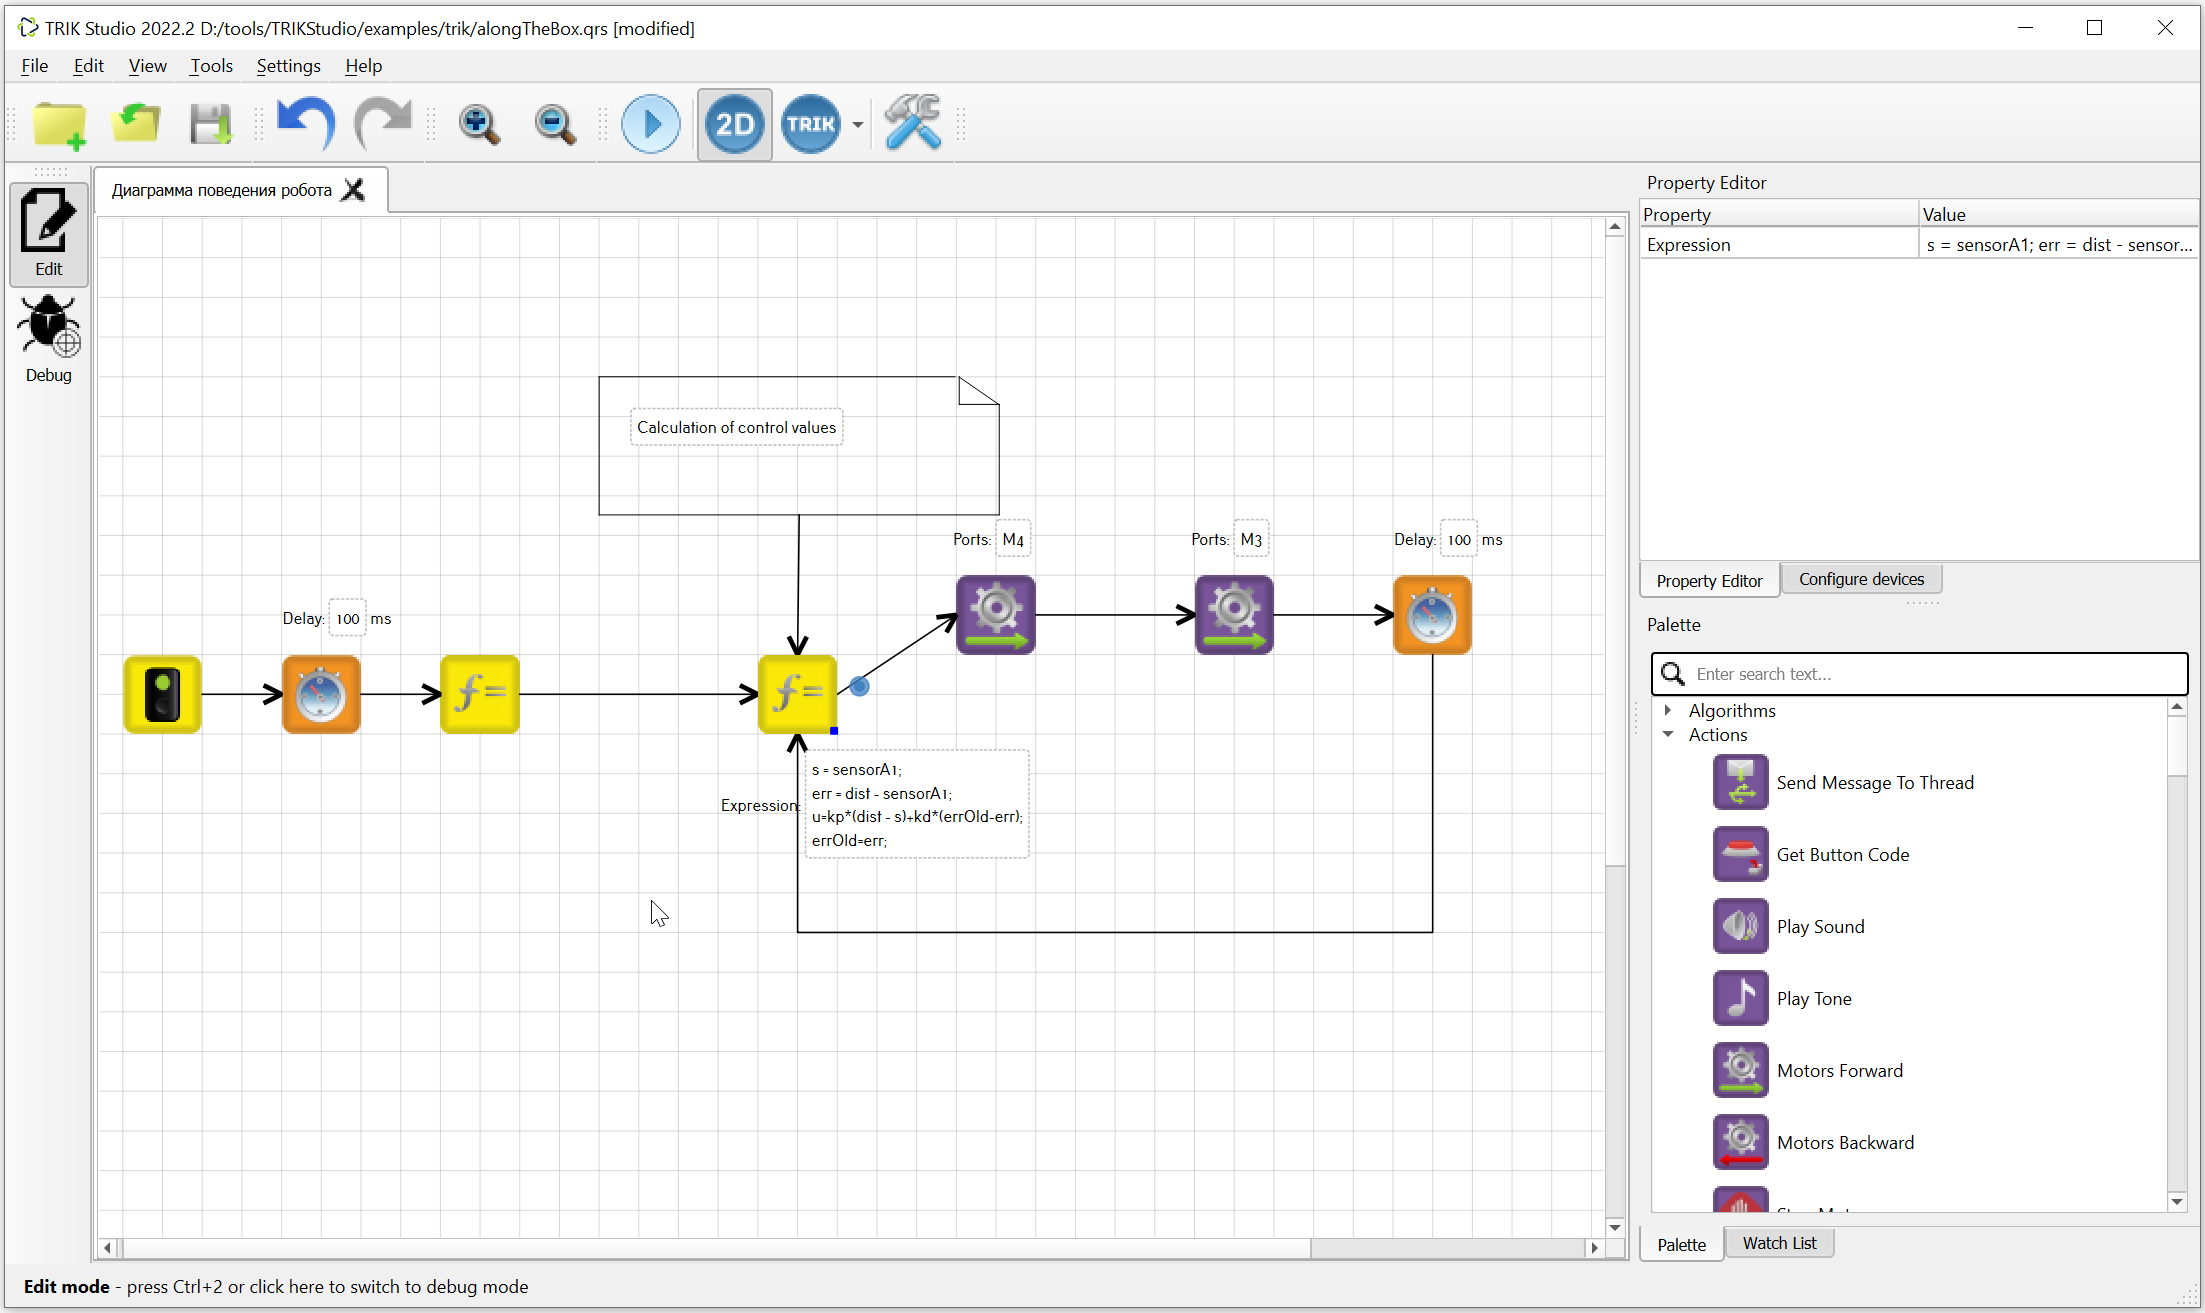
\includegraphics[width=0.9\textwidth]{trik-studio.png}
        \end{center}
    \end{frame}

    \begin{frame}
        \frametitle{DSM platforms}
        \begin{itemize}
            \item To specialize a language for a specific domain is to build a specialized tool every time
            \begin{itemize}
                \item Not feasible except for very rare special cases
            \end{itemize}
            \item Solution --- tools to create visual tools: DSM platforms
            \begin{itemize}
                \item E.g. MetaEdit+, Eclipse Sirius, QReal
            \end{itemize}
            \item They use formal definition of visual language to generate tooling
            \item But how to define visual language?
        \end{itemize}
    \end{frame}

    \begin{frame}
        \frametitle{Formal definition of visual languages}
        \begin{itemize}
            \item Metamodel --- a model of all correct models
            \begin{itemize}
                \item Much like grammar for textual languages
                \item Grammars were used for visual languages too, but rarely
            \end{itemize}
            \item Defines entities, their attributes (with types) and possible relations
            \item Metamodels can be textual and visual
            \item UML uses visual metamodel defined in UML standard
            \begin{itemize}
                \item Standalone version is known as MOF
            \end{itemize}
        \end{itemize}
    \end{frame}

    \begin{frame}
        \frametitle{Metalevels}
        \begin{center}
            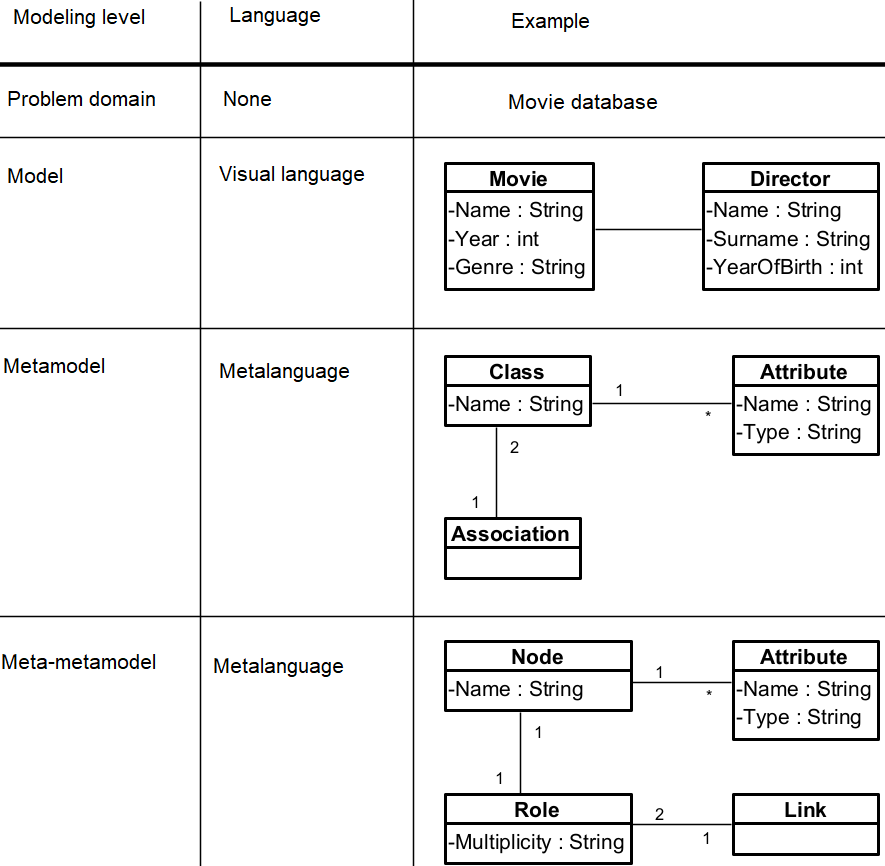
\includegraphics[width=0.5\textwidth]{metalevels-en.png}
        \end{center}
    \end{frame}

    \begin{frame}
        \frametitle{It's not that easy}
        \begin{center}
            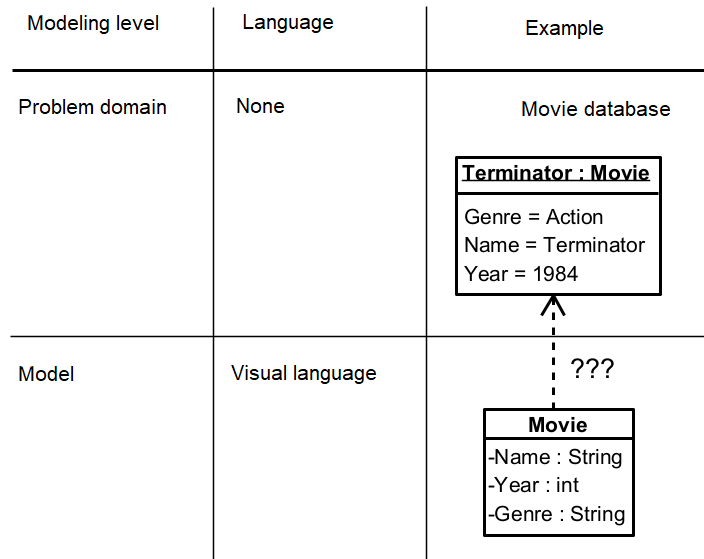
\includegraphics[width=0.4\textwidth]{terminator-en.png}
        \end{center}
        \begin{itemize}
            \item Object in UML is not an instance of a class
            \item Multi-level and deep metamodeling were invented to fix such problems
            \begin{itemize}
                \item Every model can be seen as a metamodel for a model below
                \item E.g. class diagram as a metamodel of object diagram
                \item Tools: MetaDepth, Melanee, REAL.NET
            \end{itemize}
        \end{itemize}
    \end{frame}

    \begin{frame}
        \frametitle{Visual modeling in IDEs}
        \begin{itemize}
            \item Use existing library and build ad-hoc solutions on top of it:
            \begin{itemize}
                \item IntelliJ IDEA --- yFiles
                \item Community plugins, e.g. Visual Studio Code and Diagrams.net
            \end{itemize}
            \item Create own DSM platform and build tooling with it
            \begin{itemize}
                \item Eclipse --- EMF, GMP; de-facto standard for visual languages research, can do everything, but complex 
                \item Visual Studio --- MS DSL Tools (Modeling SDK); little adoption as a standalone platform, but VS models built on top of it (kind of)
            \end{itemize}
        \end{itemize}
    \end{frame}

    \begin{frame}
        \frametitle{Example: Visual Studio Class Designer}
        \begin{center}
            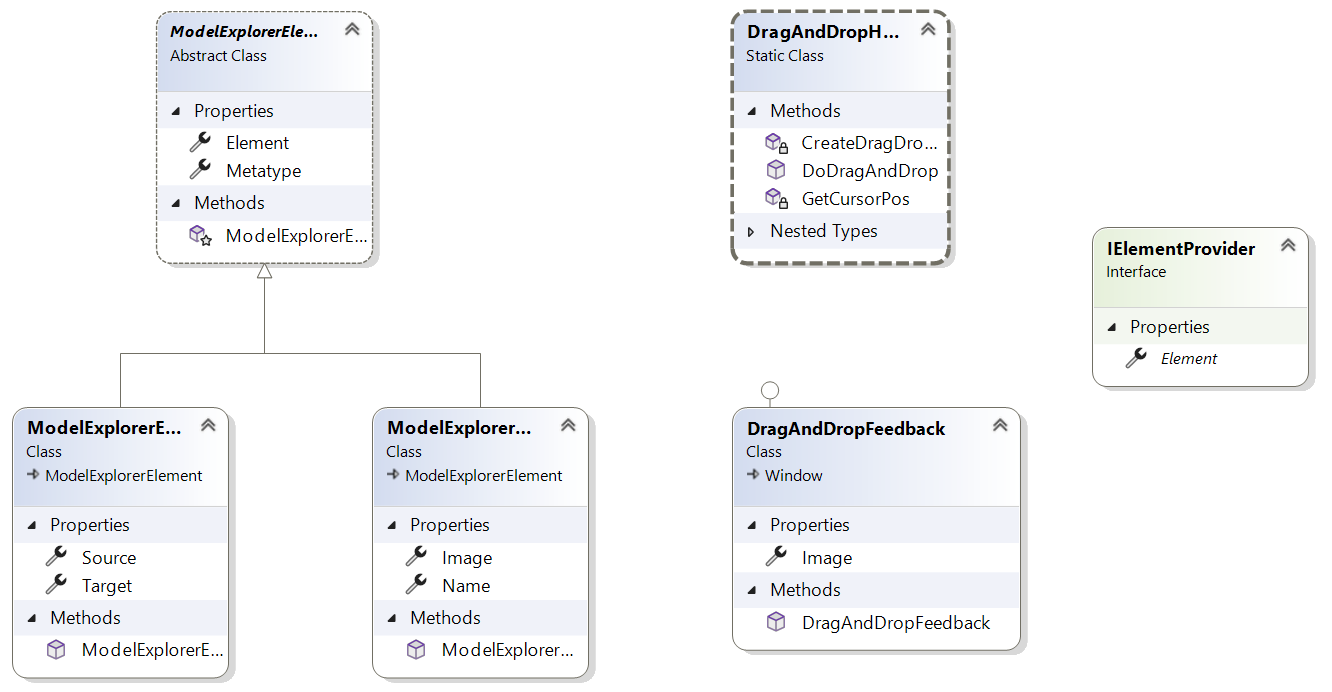
\includegraphics[width=0.7\textwidth]{visual-studio.png}
        \end{center}
    \end{frame}


    \begin{frame}
        \frametitle{Visual modeling in IDEs, problems}
        \begin{itemize}
            \item Round-trips with textual representation
            \begin{itemize}
                \item Requires something like PSI
                \item Models are considered as a view on an underlying code model, just like textual code
            \end{itemize}
            \item Usability!
            \begin{itemize}
                \item Actually, it is a general problem for diagram editors
                \item Textual code editing is much less painful
            \end{itemize}
        \end{itemize}
    \end{frame}

    \begin{frame}
        \frametitle{Visual languages in SPbU}
        \begin{itemize}
            \item RTST and earlier works (1980s) --- SDL and Algol 68, for telecommunications
            \item REAL and REAL-IT (1990s) --- UML 1.0, Visual Basic for information systems generation
            \item QReal (2005) --- UML 2.0 (at least supposed to), metamodeling
            \item QReal:Robots/TRIK Studio (2011) --- actual technology on QReal, widely spread in Russia as educational robotics tool
            \item REAL.NET (2016) --- .NET and web version, multilevel metamodeling
        \end{itemize}
    \end{frame}

    \begin{frame}
        \frametitle{Keypoints}
        \begin{itemize}
            \item A <<winter of visual modeling>> seems to be close to an end, due to need for end-user programming
            \item Visual languages support in IDEs is lacking (but present), due to low interest from programmers
            \item None of the existing IDEs support actual UML standard
            \begin{itemize}
                \item Most popular tools are only mimic UML, and do it badly
            \end{itemize}
            \item Low-code solutions integrated into light-weight IDEs seem to be interesting vector of future work
            \item Visual languages support requires effort in the fields of language theory and usability
            \item There is a need for reusable assets for support of domain-specific visual languages
        \end{itemize}
    \end{frame}

\end{document}
